%%%%%%%%%%%%%%%%%%%%%%%%%%%%%%%%%%%%%%%%%%%%%%%%%%%%%%%%%%%%%%%%%%%%%%%%%%%%%%%%%%%%%%%
%% This file was auto-generated by pandoc (https://pandoc.org) from an
%% original Microsoft Word .docx source, and then lightly edited both for
%% content and for formatting.
%%
%% However, much of the auto-generated LaTeX markup is still in place and
%% is probably repellent to a LaTeX expert's eyes. Sorry.
%%
%% The main fix-up that a future owner of this document should perform
%% is to the citations/bibliography.  The translation from Word did not auto-generate
%% a LaTeX-style bibliography. Instead, the citation numbers are, in effect,
%% hard-coded, and the Bibliography table is similarly fragile (watch what happens if
%% you remove the \newpage so that it spans a page...!
%%
%% For reference, the pandoc command to generate the .tex file from .docx was:
%%
%% pandoc -f docx -i src/ConclaveIntroductoryWhitepaperForConversion.docx -t latex -o \
%%   src/ConclaveIntroductoryWhitepaperConverted.tex -s --verbose -C --extract-media=src
%%
%% This took some trial and error.  Not 100% sure the -C option is needed.
%%
%% Build the pdf with pdflatex (run it twice)
%%%%%%%%%%%%%%%%%%%%%%%%%%%%%%%%%%%%%%%%%%%%%%%%%%%%%%%%%%%%%%%%%%%%%%%%%%%%%%%%%%%%%%%

% Options for packages loaded elsewhere
\PassOptionsToPackage{unicode}{hyperref}
\PassOptionsToPackage{hyphens}{url}
%
\documentclass[
]{article}
\usepackage{amsmath,amssymb}
\usepackage{lmodern}
\usepackage{iftex}
\ifPDFTeX
  \usepackage[T1]{fontenc}
  \usepackage[utf8]{inputenc}
  \usepackage{textcomp} % provide euro and other symbols
\else % if luatex or xetex
  \usepackage{unicode-math}
  \defaultfontfeatures{Scale=MatchLowercase}
  \defaultfontfeatures[\rmfamily]{Ligatures=TeX,Scale=1}
\fi
% Use upquote if available, for straight quotes in verbatim environments
\IfFileExists{upquote.sty}{\usepackage{upquote}}{}
\IfFileExists{microtype.sty}{% use microtype if available
  \usepackage[]{microtype}
  \UseMicrotypeSet[protrusion]{basicmath} % disable protrusion for tt fonts
}{}
\makeatletter
\@ifundefined{KOMAClassName}{% if non-KOMA class
  \IfFileExists{parskip.sty}{%
    \usepackage{parskip}
  }{% else
    \setlength{\parindent}{0pt}
    \setlength{\parskip}{6pt plus 2pt minus 1pt}}
}{% if KOMA class
  \KOMAoptions{parskip=half}}
\makeatother
\usepackage{xcolor}
\IfFileExists{xurl.sty}{\usepackage{xurl}}{} % add URL line breaks if available
\IfFileExists{bookmark.sty}{\usepackage{bookmark}}{\usepackage{hyperref}}
\hypersetup{
  pdftitle={Conclave: An Introduction},
  hidelinks,
  pdfcreator={LaTeX via pandoc}}
\urlstyle{same} % disable monospaced font for URLs
\usepackage{longtable,booktabs,array}
\usepackage{calc} % for calculating minipage widths
% Correct order of tables after \paragraph or \subparagraph
\usepackage{etoolbox}
\makeatletter
\patchcmd\longtable{\par}{\if@noskipsec\mbox{}\fi\par}{}{}
\makeatother
% Allow footnotes in longtable head/foot
\IfFileExists{footnotehyper.sty}{\usepackage{footnotehyper}}{\usepackage{footnote}}
\makesavenoteenv{longtable}
\usepackage{graphicx}
\makeatletter
\def\maxwidth{\ifdim\Gin@nat@width>\linewidth\linewidth\else\Gin@nat@width\fi}
\def\maxheight{\ifdim\Gin@nat@height>\textheight\textheight\else\Gin@nat@height\fi}
\makeatother
% Scale images if necessary, so that they will not overflow the page
% margins by default, and it is still possible to overwrite the defaults
% using explicit options in \includegraphics[width, height, ...]{}
\setkeys{Gin}{width=\maxwidth,height=\maxheight,keepaspectratio}
% Set default figure placement to htbp
\makeatletter
\def\fps@figure{htbp}
\makeatother
\setlength{\emergencystretch}{3em} % prevent overfull lines
\providecommand{\tightlist}{%
  \setlength{\itemsep}{0pt}\setlength{\parskip}{0pt}}
\setcounter{secnumdepth}{-\maxdimen} % remove section numbering
\ifLuaTeX
  \usepackage{selnolig}  % disable illegal ligatures
\fi

\title{Conclave: An Introduction}
\author{Richard Gendal Brown\footnote{\href{mailto:richard@r3.com}{\nolinkurl{richard@r3.com}}}}
\date{December 2021}

\begin{document}
\maketitle

\hypertarget{abstract}{%
\section{Abstract}\label{abstract}}

We present Conclave: a platform for the rapid development and execution
of `privacy-first' applications; and a set of privacy-first cloud
services that are themselves built using the Conclave platform. Conclave
applications can remotely `attest' to users how their information will
be handled and which parties, if any, can influence this execution or
access the data. Building on the power of Trusted Execution
Environments, Conclave puts the power of hardware roots of trust into
the hands of mainstream developers and their users.

\newpage
\hypertarget{contents}{%
\tableofcontents \label{contents}}


\newpage
\hypertarget{executive-summary}{%
\section{Executive Summary}\label{executive-summary}}

Privacy-first applications and services can prove how they will process
their inputs, can prove that their outputs are the result of a specific
program, and their execution cannot be observed or tampered with.

Conclave enables developers to write privacy-first applications with ease,
by putting the power of Trusted Execution Environments such as Intel
SGX {[}1{]} into a form they can exploit using the productive high-level
languages they're already using to develop their existing solutions.
This focus on productivity stands in contrast to the learning curve
associated with competing software-based cryptographic approaches.
Conclave further distinguishes itself through the speed with which
developers familiar with languages such as Java, JavaScript, Kotlin and
Python can develop compelling, privacy-first applications, providing
very high level APIs that solve messaging and storage problems that
inhibit adoption of competing TEE platforms. Integrating tightly with
public cloud platforms, Conclave enables users to build, deploy and
integrate privacy-first services at scale.

We expect Conclave to be of particular benefit to firms who process
sensitive data on behalf of other firms, and to those seeking
reassurance about how their data will be handled when shared with cloud
services. We also expect it to be beneficial to firms where sharing data
between departments or across borders is presently difficult.

Conclave is likely also to find adoption amongst those who have explored
software-based privacy-enhancing cryptographic techniques such as
Zero-Knowledge Proofs, Fully Homomorphic Encryption, and Secure
Multi-Party Computation but found the complexity and lack of
general-purpose tools an inhibitor to success.

Conclave's ability to support `privacy-first' application derives from
its ability to provably execute code that runs as designed and cannot be
tampered with. Privacy is the obvious and most immediate application for
such a capability, and is the focus of this paper. However, we also
anticipate Conclave being used in time to disrupt entirely different
markets, through its more general ability to eliminate certain types of
trusted third parties through the substitution of attestably
tamper-resistant code.

Conclave heralds the mainstream era of `privacy-first' computation.

\hypertarget{motivation-and-background}{%
\section{Motivation and Background}\label{motivation-and-background}}

The technical heart of the `data privacy and control' problem is that
anybody in control of a computer is able to observe the data it has
access to, and can arbitrarily modify what the computer does with that
data.

This means that if you send a piece of information to somebody else's
computer, you must assume that this person can both \emph{see} this
information and can configure their computer to \emph{do} anything with
it they choose.

``Privacy-enhancing techniques'', both software- and hardware-based,
solve this problem, and have been widely available for some time. But it
is only with the advent of Conclave that it has become a realistic
proposition for mainstream businesses to consider applying these
techniques to solve their real-world problems.

\hypertarget{real-world-privacy-problems-conclave-can-solve}{%
\subsection{Real-World Privacy Problems Conclave Can
Solve}\label{real-world-privacy-problems-conclave-can-solve}}

Here we provide motivation for what follows by outlining five otherwise
difficult privacy-related business problems that can now be easily
solved with Conclave:

\begin{itemize}
\item
  Train a machine learning model in the cloud without the cloud provider
  seeing your training data
\item
  Collaborate with peers in your industry to identify suspicious
  patterns of behaviour across your customer sets, without any
  competitor or third party actually having access to your proprietary
  data
\item
  Build an online exchange that can prove to buyers and sellers that
  sophisticated insiders cannot `front run' their trades
\item
  Run online opinion polls whose participants can be sure their
  responses will never be revealed
\item
  Implement a `burst-mode' cloud-hosted computation feature to a mobile
  app with the same privacy and integrity assurances as code that runs
  locally
\end{itemize}

And, as discussed in the introduction, Conclave can also be used to
disintermediate any business model that exists solely because of an
historical inability to remotely verify that a third party has done what
they said they would. For example, Conclave could be used to implement
an entirely decentralised system for verifying control of websites, and
issuing of certificates.

\hypertarget{background}{%
\section{Background}\label{background}}

The spread of the Internet into all facets of life in the first two
decades of the 2000s has created enormous value for billions of people.
But in the breakneck race to connect everybody and everything, the IT
industry has been less quick to ensure the data being so freely shared
was sufficiently protected when in the hands of others.

So it is perhaps not surprising how many of the most urgent public
policy issues of the early 2020s are a direct consequence of this
revolution. And it is striking how many of today's technology policy
issues share a single cause: the explosion in the movement and sharing
of information amongst firms and individuals has vastly outpaced our
ability to control what happens to that information when it leaves the
control of its owner.

Consider this list of technology policy issues on the agendas of most
developed nations at the start of the 2020s:

\begin{itemize}
\item
  Social networks are accused of misusing users' personal data for
  corporate gain {[}2{]}.
\item
  Advertisers, and the large technology firms whose platforms display
  their ads, are accused of tracking users without their knowledge, and
  of inappropriately combining disparate datasets to violate users'
  reasonable expectations that different online behaviours and personas
  can be kept separate {[}3{]}.
\item
  Firms of all sorts are accused of using data they obtained about an
  individual for one purpose to pursue unrelated business goals, without
  informed consent {[}4{]}.
\item
  Data that firms legitimately capture about users is often stored or
  processed with insufficiently strong controls, leading to data loss or
  exposure, by malicious outsiders or rogue insiders {[}5{]}.
\item
  Firms frequently wish to share data with other firms, but are unable
  to control this data once it leaves their systems. They fear the
  resulting liability, and so forego otherwise promising opportunities
  for themselves or their customers.
\end{itemize}

These issues all share a single cause: today's networked economy
requires individuals and firms to share data with third parties or other
parts of the same firm on an unprecedented scale, yet today's technology
provides no way to control how that data is then used, or for what
purpose.

The blunt reality is that once you have shared a piece of information
with a third party, they can do whatever they like with it. The only
things constraining them are `soft' controls: reputation, regulation and
contract law. The internet revolution has made it extraordinarily easy
and cheap to share information, but has provided no comparably powerful
tools to control the monster we unleashed.

In what follows, we begin by enumerating three reasons individuals and
firms share data with third parties. We then introduce hardware Trusted
Execution Environments (TEEs) as a maturing, but difficult to use,
technology that can enable data sharing with privacy. The Conclave
platform is then introduced as an easy and accessible toolkit and set of
cloud services for harnessing TEEs, thus unlocking their potential.

\hypertarget{the-three-reasons-we-share-data}{%
\section{The Three Reasons We Share
Data}\label{the-three-reasons-we-share-data}}

There are at least three distinct reasons we share information with
third parties:

\begin{itemize}
\item
  `Outsourced Computation'

  \begin{itemize}
  \item
    Example: cloud computing
  \end{itemize}
\item
  `Independent Verification of Information'

  \begin{itemize}
  \item
    Example: demanding proof that a service consumer is old enough
  \end{itemize}
\item
  `Multi-Party Collaboration'

  \begin{itemize}
  \item
    Example: buyers and sellers utilising a centralised exchange to
    facilitate trade
  \end{itemize}
\end{itemize}

In what follows, we explore these scenarios to elucidate their
fundamental characteristics, and identify requirements a
privacy-enhancing technology would need to meet in order to improve the
privacy of each type of service.

\hypertarget{outsourced-computation}{%
\subsection{Outsourced Computation}\label{outsourced-computation}}

Outsourced computation is an increasingly common way in which firms and
individuals experience computing services today:

\begin{itemize}
\item
  IT administrators run workloads on cloud Infrastructure as a Service
  (IaaS) services to benefit from economies of scale and variable
  pricing.
\item
  Developers utilise cloud Platform as a Service (PaaS) offerings, such
  as managed database services or `function as a service', to eliminate
  the need to run their own infrastructure for commoditised components
  of their solutions.
\item
  Business people increasingly rely on Software as a Service (SaaS)
  offerings, such as customer relationship management or enterprise
  resource planning.
\end{itemize}

\begin{figure}
  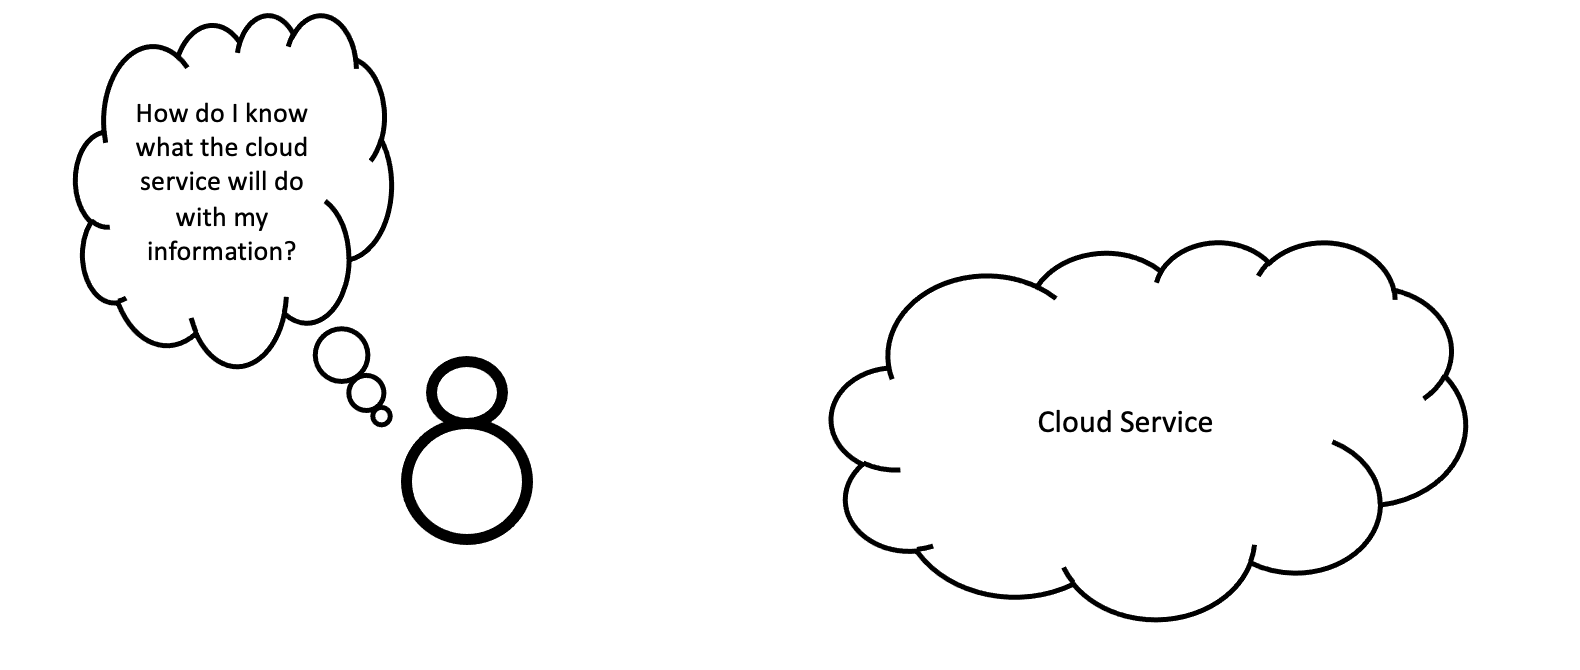
\includegraphics[width=5.0625in,height=2.14679in]{src/media/image1.png}
  \caption{When you share information with a third party, traditional
technology provides no assurances over what that party can do with the
information they receive}
  \label{image1}
\end{figure}

These scenarios can all be thought of as `outsourced computation' and
share the property that the consumer is trusting their provider
completely, as depicted in Figure \ref{image1}. There is nothing today at a
technological level that prevents the cloud provider from viewing all
the consumer's information or tampering with how the service works,
whether deliberately or inadvertently, perhaps owing to a hack or rogue
insider. And this observation is intrinsic to how such services operate
today. For example, a social media site needs to be able to know who
your friends are if it is to show you stories about them. A bank needs
to know what you've spent money on if it is to produce accurate
statements.

\hypertarget{independent-verification-of-information}{%
\subsection{Independent Verification of
Information}\label{independent-verification-of-information}}

Another reason one party shares information with another is because that
party wishes to verify that a particular fact is true.

In the real world, for example, a nightclub bouncer may wish to know
that a guest is legally old enough to enter. Or the user of a web
browser may wish to know that the site to which it is connected is owned
by the firm the site claims to represent. In the world of blockchains,
the recipient of a payment transaction wishes to know that the `coins'
they are receiving actually exist.

It often turns out that the fact being asserted, or verified, is not
particularly sensitive. However, the only available \emph{evidence} that
can be independently verified may contain far more information than the
minimal fact in question.

For example, as shown in Figure \ref{image2}, a physical passport would enable a
bouncer to verify I am over eighteen years old. But the bouncer would
also learn my actual age, full name, nationality and all the countries I
visited in recent years.
\begin{figure}
  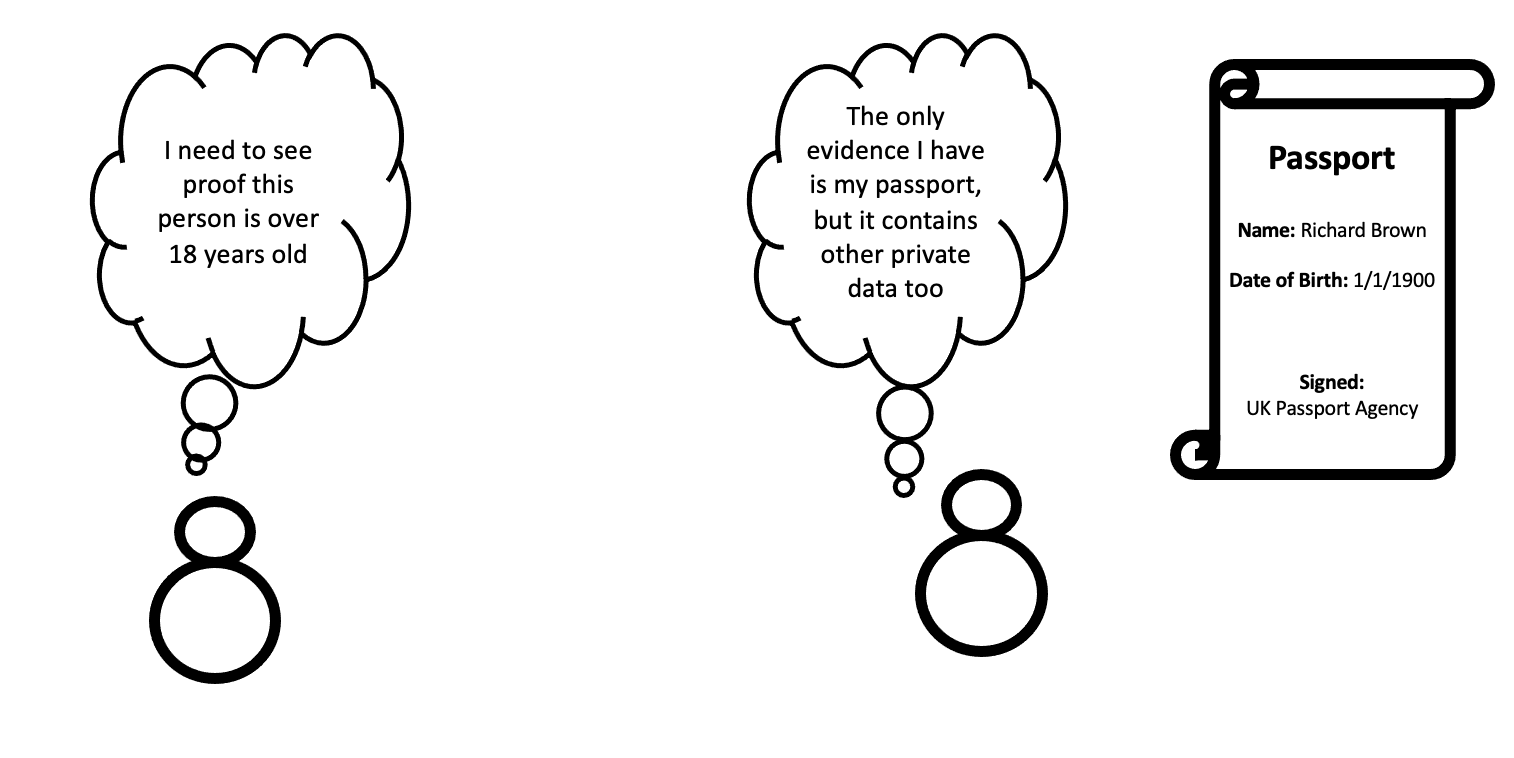
\includegraphics[width=5.40789in,height=2.70754in]{src/media/image2.png}
  \caption{In many situations it is necessary to `prove' a fact to a third
party, but without revealing the full document that provides the evidence}
  \label{image2}
\end{figure}

In the blockchain world, the recipient of a payment transaction can
verify without reliance on any third party whatsoever that the money
they have received exists and is theirs. But to do this they must
analyse all the historic blocks on the blockchain to verify that the
coins really were correctly mined at some point in the past, and that
value has been conserved ever since. But this means the recipient also
learns a great deal about the history of the coin, which could enable
them to learn something about other participants on the network.

And these examples are typical. Very often, the only available
`evidence' that a verifier can rely on reveals far more than they
actually need to know.

So we find ourselves sharing lots of information with third parties,
purely because of this `impedance mismatch' between what they need to
verify and the evidence we possess that can prove this fact. This will
be increasingly difficult to justify to regulators or other third
parties, especially as they become increasingly aware that technology
solutions to this problem now exist.

\hypertarget{multi-party-collaboration}{%
\subsection{\texorpdfstring{Multi-Party Collaboration
}{Multi-Party Collaboration }}\label{multi-party-collaboration}}

The third major reason for sharing information with a third party is
because many parties want to achieve some business outcome but none of
them possess sufficient information by themselves to do this, as
depicted in Figure \ref{image3}. And so the parties have to `pool' their
information in some way.
\begin{figure}
  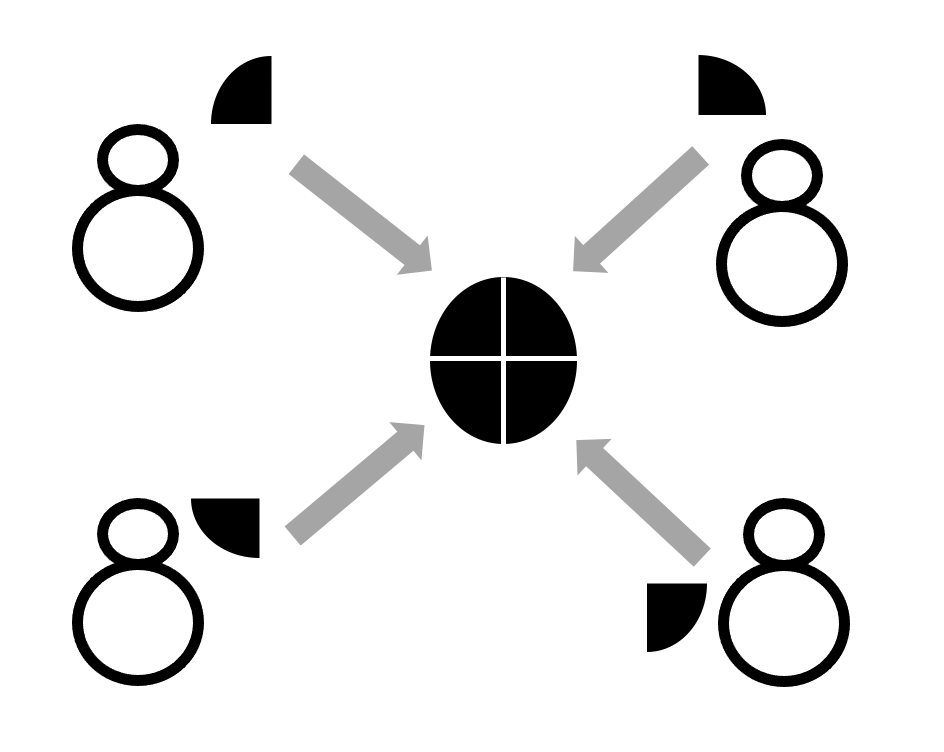
\includegraphics[width=3.46167in,height=2.75744in]{src/media/image3.png}
  \caption{Very often in business, different parties possess a piece of
  the information `jigsaw', yet there is nobody they trust to assemble the
  full picture}
  \label{image3}
\end{figure}

For example, if I wish to sell some stock I own, how do I find somebody
who might be interested in buying it? If I need to hire a new CTO for my
firm, how do I find out what the current market rates are in my
industry? If I'm processing an insurance claim how do I know if the
customer has fraudulently filed a similar claim with another insurer?

Furthermore, the emergence of Machine Learning as a mainstream
technology has revealed important situations where the best results
depend on multiple firms being able to share data securely. For example,
one firm may wish to train their model on data owned by another whilst
being able to demonstrate to the data owner that their data will not be
used for any other purpose. In other situations, multiple firms would
like to benefit from models that could be trained on their joint
datasets, but without any firm gaining sight of any other firm's
information.

In all these cases, there is a natural non-technical solution: a
centralised third party can provide a service within which each
participant shares their own data so that the overall dataset can be
pooled and processed. In the share trading case, we call this third
party a stock exchange. For the salary data case, we rely on `market
benchmark' firms. And insurers rely on industry-operated shared
databases, where regulation allows.

However, in some cases, regulation does \emph{not} allow this
information to be pooled in a way that could render sensitive
information open to attackers or other third parties. And even when such
solutions exist (eg stock exchanges and data brokers), these entities
tend to become natural monopolies, or oligopolies, with strong pricing
power over their customers and, in some cases, an incentive to pursue
business models counter to the interests of the participants who
provided the data in the first place.

But what if there was a way to collectively pool data to solve these
sorts of problems but in a way that prevented the central operator from
exploiting their position of power or from learning anything about the
aggregated data set?

\hypertarget{discussion-different-scenarios-same-problem}{%
\subsection{Discussion: Different Scenarios, Same
Problem}\label{discussion-different-scenarios-same-problem}}

It may not be obvious at first sight, but these problems all have a
common cause: \emph{you cannot trust somebody else's computer}.

\begin{itemize}
\item
  In the first case -- outsourced computation -- you can't assume the
  cloud provider won't misuse your data
\item
  In the second case -- independent verification -- you have to share
  the full evidence for a fact because somebody else can't simply trust
  your computer if it says ``I've verified the passport for you and it's
  OK''. You could have programmed your computer to lie!
\item
  And in the third case -- multiparty computation -- the operator of the
  pooled data service has full visibility of the entire market,
  everybody's salaries or all insurance claims in a market.
\end{itemize}

But what if you \emph{could} sometimes trust somebody else's computer?
What if we \emph{could} write applications whose owners \emph{cannot}
tamper with them or observe their execution? What if an application
\emph{could} process data you are not entitled to see yet you could
trust the results that are provided at the end?

If such a system existed and could be adopted at scale then each and
every one of the public policy issues listed above could be addressed.
Data owners would regain control of their information. They could verify
what will happen to their data -- and, by extension, what therefore will
\emph{not} happen to it -- \emph{before} sending it for processing. And
if somebody else's computer told them a fact had been verified, they
could believe it.

We might name systems that work this way as being `privacy-first.' And
it is likely we will look back on the early decades of the 2000s with
shock: ``you routinely shared sensitive data with third parties with no
technological controls over what they could do with it? What were you
thinking?''

It should be noted that various cryptographic technologies that can meet
the requirements above already exist. Some techniques rely on advanced
mathematics, implemented in software. At the time of writing, they
remain specialised (as opposed to generally applicable) and require
advanced mathematical and cryptographic skills. As such, they are not
yet ready for mainstream adoption. Hardware-based `Trusted Execution
Environments', by contrast, are relatively mature, but a usability and
productivity gap remains. It is this gap that Conclave fills.

In what follows, we briefly introduce the hardware-enabled approach to
privacy-enhancement, before introducing Conclave and its unique approach
to putting these technologies into the hands of regular developers.

\hypertarget{hardware-based-privacy-enhancing-techniques}{%
\section{Hardware-Based Privacy-Enhancing
Techniques}\label{hardware-based-privacy-enhancing-techniques}}

Since the dawn of modern computing, computers have been designed on the
basis that they exist to serve their owners. And CPUs reflect this
assumption. They enable creation of systems consisting of multiple
``unprivileged'' coexisting applications, overseen by a ``privileged''
supervisor (which we call an operating system kernel and hypervisor,
where present), which is responsible for mediating their access to
scarce real-world resources, and for protecting the integrity of the
system. This situation is depicted in Figure \ref{image4}, where a client is
interacting with an application hosted on a traditional server. The
application is fully under the control of the supervisor, which is under
the control of the owner of the server. The client has no way of knowing
what will actually happen to any data shared with the server.

\begin{figure}
  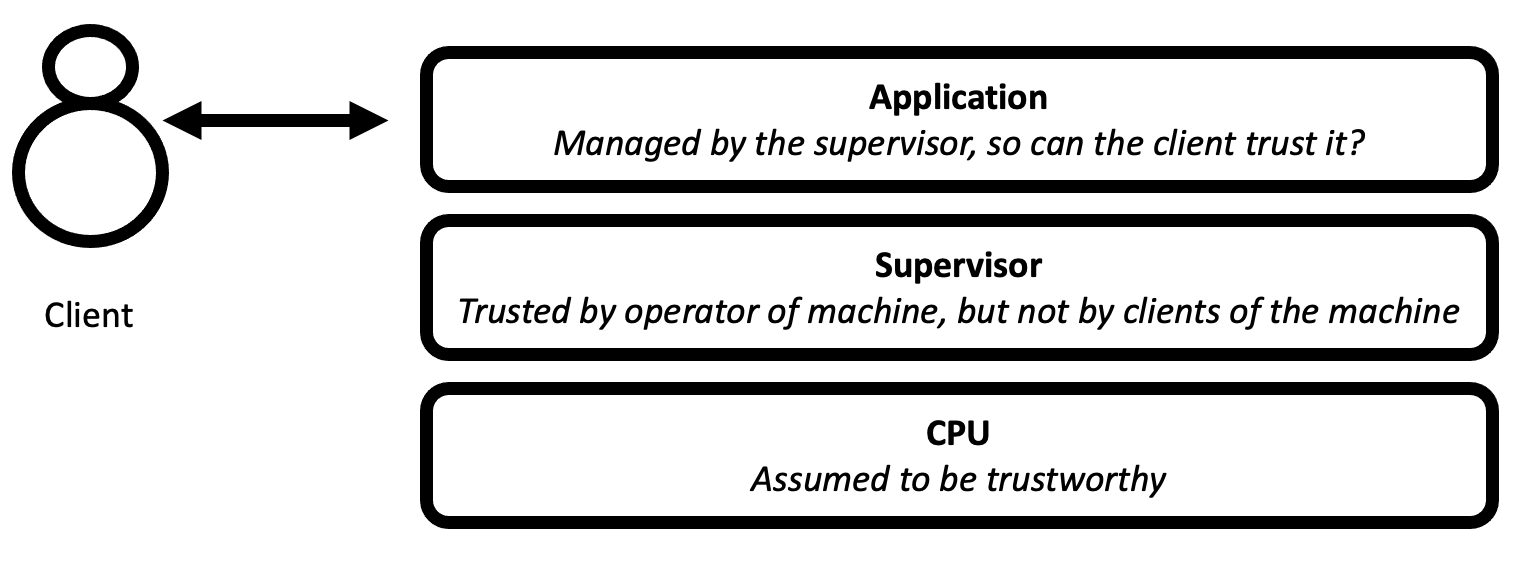
\includegraphics[width=4.8886in,height=1.87252in]{src/media/image4.png}
  \caption{In a traditional computing environment, the supervisor (aka
  operating system kernel and hypervisor if present) is trusted by and
  under the control of the owner of the machine, and enjoys a privileged
  position. It has complete control over the applications it hosts.}
  \label{image4}
\end{figure}


In this model, the operating system is `all-powerful', acting benignly
on behalf of the owner of the system. Applications are presumed to be
buggy and maybe even malicious. The operating system is thus granted
supremacy over the applications, which are assumed to be the source of
threats.

And this explains why you cannot trust a service running on somebody
else's computer: the service isn't in full control; it is merely an
application running on that computer. And it exists and operates at the
pleasure of the operating system kernel, which controls \emph{and sees}
everything the application does. And since the operating system is under
the control of the owner of the computer, the service's users must
assume the owner of the computer can see their data and arbitrarily
tamper with the application's business logic. If you trust the owner of
the computer on which the service runs, then all is good. But if you
don't -- or worry about what may happen if they are hacked -- then we
have a problem.

The idea behind ``Trusted Execution Environments'', or TEEs {[}9{]} --
the hardware approach to privacy-first computing -- is to turn this
design on its head. A modern TEE, such as Intel SGX, allows an
application to escape from the snooping eyes and capricious hands of the
operating system. Such applications still rely on the cooperation of the
operating system to run and communicate with the outside world, but the
operating system is prevented -- at the physical hardware level -- from
looking at the memory being used by the application or from changing the
application's business logic. And the hardware is able to create a
digital `certificate' that \emph{proves} the application is running in
this mode.

This model is depicted in Figure \ref{image5}, where we see application code called
an `enclave' running in a mode where the supervisor can \emph{not}
observe what it is doing and can \emph{not} tamper with its execution.

\begin{figure}
  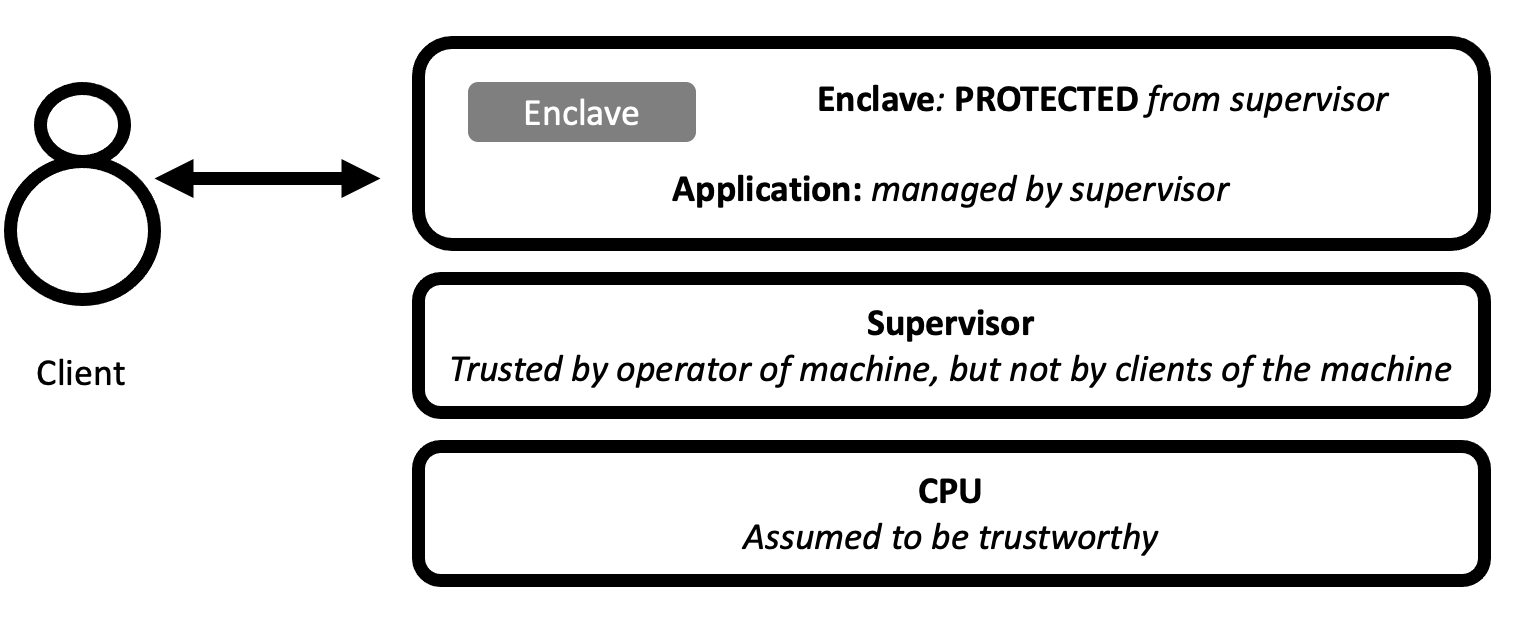
\includegraphics[width=4.80357in,height=1.99172in]{src/media/image5.png}
  \caption{A Trusted Execution Environment such as Intel SGX allows the
  creation of so-called 'enclaves', which are application code that cannot
  be tampered with - or observed executing - by the supervisor. As such,
    the owner of the server is "locked out"
  }
  \label{image5}
\end{figure}

Applications running on a Trusted Execution Environment, which we call
enclaves, can ask the underlying hardware to produce a signed document
for clients to review, which we call an `attestation', which can be
thought of as making the following statement:

\emph{``To whomever this may concern: this application is running on a
fully patched system in a mode whereby its memory is encrypted and its
code is tamper-resistant. This application possesses a private key,
whose public portion is as follows. I attest that no other application
or system has access to this key and, as such, any data you encrypt with
this key can only be accessed and operated on by the application
matching the description above. Signed Intel/AMD/ARM/IBM''}

The exact details of the `report' vary between manufacturers and
use-cases but the principle of a hardware-rooted `remote attestation' is
at the heart of the concept: the hardware, in effect, makes a `promise'
that a particular piece of code is running and that the operating system
and the rest of the hosting system has been locked out.

This concept can be used to address \emph{all three} of the privacy
requirements outlined above:

\textbf{Outsourced Computation}

If you have some business logic that you would like a third party to
execute on your behalf then the remote attestation process allows you to
verify that the third party cannot access your data, because the
decryption key is not available to them. Importantly, the TEE approach
goes further than the equivalent software-only technique: unlike Fully
Homomorphic Encryption, a software-based technique, a TEE can assure you
that not only is your data out of the reach of the operator, but it can
also assure you precisely which code is running, or that the code has
been signed by an entity you specify. In short, TEEs allow you to run
workloads on somebody else's computer in a way that lets you verify they
can neither \emph{observe} the data nor \emph{lie} about how it is
processed\footnote{One special case of `outsourced computation' arises
  when a firm such as a bank wishes to run an existing workload in the
  cloud, where the only assurance they seek is that the cloud operator
  cannot tamper with it. This model is sometimes called `lift and
  shift.' Unlike other uses of TEEs, where the ultimate consumer of a
  service receives assurances about how their data will be processed,
  `lift and shift' focuses only on the relationship between the
  application owner and their cloud provider; the promise does not
  extend to their users. This is a compelling value proposition to any
  large firm with sensitive workloads that they wish to move to the
  cloud, and all major cloud vendors will increasingly offer this as a
  core service. However, Conclave does not target this category.}.

\textbf{Independent Verification}

Imagine you have a digital birth certificate and want to prove to
somebody that you are over eighteen years old. Can you use a trusted
execution environment to solve this problem? Yes. You could write a
simple application that can verify the signature on a digital birth
certificate and extract the date of birth and name fields. The
application then checks the date of birth was at least eighteen years
before a given date and, if so, generates and signs a \emph{new} data
structure which states:

\emph{``A birth certificate issued by a key known to be owned by
\textless The UK Government\textgreater{} for name \textless Richard
Gendal Brown\textgreater{} confirmed that this person was at least
\textless Eighteen\textgreater{} years old as of \textless Thursday 25
November 2021\textgreater.''}

A party relying on this information learns nothing other than the
proving party's age, exactly as we require. Importantly, this also
demonstrates that it is thus possible for a Trusted Execution
Environment to achieve the same outcomes as a zero knowledge proof, a
sophisticated but complex software-based technique.

\textbf{Multi-Party Computation}

Finally, it should hopefully be clear that if you possess a TEE, then
the `outsourced computation' scenario can be easily generalised to the
case where \emph{multiple} parties are sharing data with the
privacy-protected application.

\hypertarget{overview-of-conclave}{%
\section{Overview of Conclave}\label{overview-of-conclave}}

Conclave is a software development kit and suite of complementary cloud
services for the rapid development of privacy-first applications through
the use of hardware Trusted Execution Environments.

Users of Conclave can use high-level languages such as Java, Kotlin and
JavaScript to develop hardware-secured services which can prove how the
service will process their inputs, can prove that the service's outputs
are the result of a specific program, whose execution cannot be observed
or tampered with, and which can \emph{remotely attest} to their users
that this is the case. We say such services are `privacy-first'.

Conclave compares favourably to many other Software Development Kits
(SDKs) that developers could use to exploit TEEs, whose APIs are often
low-level and require deep knowledge of the underlying hardware. By
contrast, Conclave differentiates itself against most of these SDKs as
follows:

\begin{itemize}
\item
  Conclave's API, the Mail library in particular, is high-level,
  completely abstracts the underlying hardware, and makes a large number
  of decisions on behalf of developers so as to reduce their cognitive
  burden, including to entirely eliminate certain classes of security
  issues common to naïve implementations.
\item
  As a result, it can be extremely quick to develop applications on
  Conclave. Anecdotes from developers who have used both Conclave Core
  and competing SDKs suggest that it may be as much as an order of
  magnitude more productive.
\item
  Conclave also supports a wide range of programming languages,
  including Java, JavaScript, Kotlin and Python, and more, including R,
  Ruby and others can be added easily.
\item
  Conclave Core is also one of the few SDKs that tightly integrates with
  a complementary cloud offering, providing a seamless path from
  development to deployment, and including features that enable
  workloads to migrate between cloud servers transparently, something
  that is not available `out of the box' from the underlying hardware.
\item
  And Conclave Cloud, in turn, distinguishes itself against its
  competitors through the ease with which services can be deployed, its
  integration with Conclave Core (providing a bridge between the two
  models of application development) and the speed at which it can
  deliver new services, as a result of it being built itself using
  Conclave Core.
\end{itemize}

As a result, Conclave is dramatically easier and more productive than
any existing enclave authoring solution, allowing users to focus on
solving their business problem, not the technical details associated
with securely deploying Trusted Execution Environments.

Conclave can be used directly to develop and deploy valuable
customer-facing applications. And it can be used as the foundation of
higher-level cloud-deployed developer services, such as confidential
databases, lambda-style functions, or search, from which other
applications can be constructed.

In what follows, we first introduce the high level components of the
\emph{Conclave Core} platform, how they combine to create a simple
programming model, and how some of the product features are implemented
at a technical level. We then summarise the services that comprise
\emph{Conclave Cloud}, the set of cloud-based services R3, the creators
of Conclave, have developed, or may deliver in the future.

\hypertarget{conclave-core}{%
\subsection{\texorpdfstring{Conclave Core
}{Conclave Core }}\label{conclave-core}}

Conclave Core is a platform for developing and deploying privacy-first
services. A typical Conclave deployment looks very much like \emph{any}
application: a server, in the form of a Java Virtual Machine, hosts the
application code, and clients running on other computers connect to the
server. Importantly, and as we describe in more detail below, the
business logic can be written in a surprisingly wide range of languages,
not just Java.

However, unlike other server applications, \emph{Conclave} applications,
which we call \emph{enclaves}, are protected from owner of the server on
which they run, and Conclave \emph{clients} have the ability to verify
that everything is working as intended.

\begin{figure}
  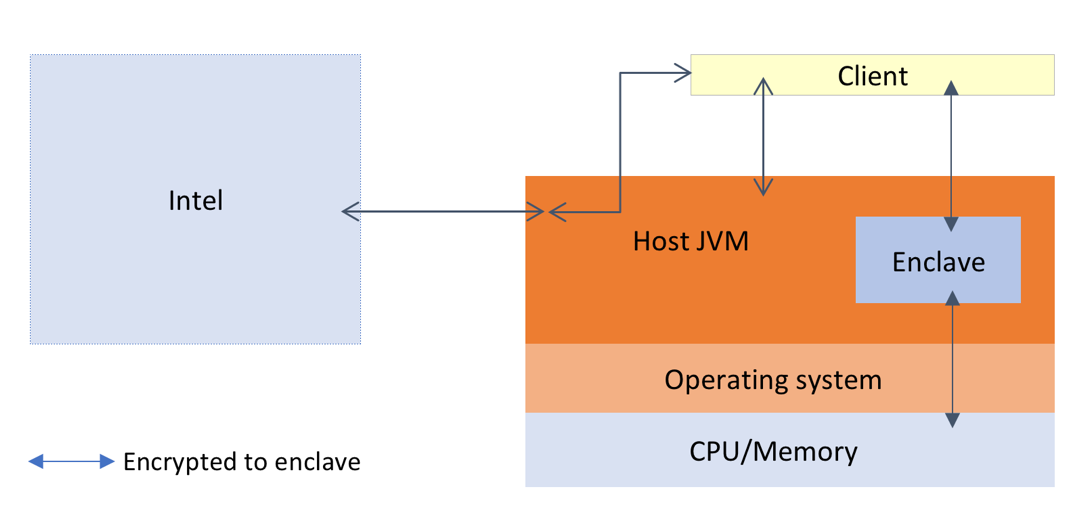
\includegraphics[width=4.91964in,height=2.34692in]{src/media/image6.png}
  \caption{Conclave Core makes it easy to develop secure enclaves that can
  run on Trusted Execution Environments such as Intel SGX. Conclave
  enclaves are hosted in JVMs but can themselves be written in a range of
  languages
  }
  \label{image7}
\end{figure}


In Figure \ref{image7}, we see a high-level architecture overview of a Conclave
deployment. Conclave Core takes code written in, for example, Java,
JavaScript, Kotlin, Python and transforms it into an enclave that can
run in a Trusted Execution Environment. This enclave is \emph{hosted} in
a JVM, which runs as an application on an otherwise untrusted machine.
In this section, we dig into these concepts.

\hypertarget{enclave}{%
\subsubsection{Enclave}\label{enclave}}

The heart of a Conclave application, where sensitive business logic and
data is contained, is called an \emph{enclave}. Enclaves can be written
in -- or dynamically execute -- a variety of high-level languages.
Enclaves have the unique property that they are protected from the
computer on which they run. This means that nothing, including the
operating system, hypervisor or BIOS, can tamper with the enclave's
business logic or observe the data on which it is operating.

This stands in contrast to regular application code running on a server,
where the operating system and other privileged components have full
control over the application, including the ability to alter its
business logic without detection, and to inspect all data that the
application has access to.

Importantly, enclaves also have the ability to obtain an unforgeable
cryptographic proof from the underlying hardware that they are indeed
running in this protected mode, and that a particular piece of code is
being executed. This means that enclaves can be used to provide services
that not only process data confidentially and without the risk of
tampering, but which can \emph{prove} that this is the case to their
users.

However, this ability also brings some constraints. In particular,
enclaves must assume that the hardware upon which they are running is
under the control of an attacker, perhaps who also has control of the
operating system. Therefore, enclaves operate in an environment where
any interaction with storage or network could be observed or manipulated
by an adversary. To model this and make it easier for programmers to
reason about the otherwise quite complex situation, enclaves do not have
unfettered access to the hardware on which they run. Instead, enclaves,
which are native Linux libraries, are themselves `hosted' in a
\emph{regular} and hence untrusted operating system process (the Java
Virtual Machine referred to above), with which the enclave
\emph{cooperates} to facilitate communication with the outside world.
One of the most important aspects of Conclave's design is how the
interaction between the Enclave and its host is implemented in order to
ensure the security assurances of the platform are delivered in
practice. Furthermore, Conclave's `Mail' API and `Common Host'
significantly simplifies development effort and reduces the required
expertise.

At an implementation level, Conclave allows developers to write enclaves
in any JVM-supported language, and enclaves themselves can be configured
to dynamically load code written in a far broader range of languages at
runtime, including JavaScript and Python. Additional languages can be
added in the future.

At build-time, Conclave compiles the application to an Intel-SGX
compatible native library utilising the GraalVM {[}10{]} \emph{`Native
Image'} system. This native library is then linked with the Conclave
trusted enclave runtime and packaged into an SGX enclave binary. This
enclave binary is then loaded into a regular Java Virtual Machine, which
itself is running in unprotected memory. This unprotected, and hence
unconstrained, JVM is responsible for managing the enclave's lifecycle
and connecting it to the outside world.

Conclave's ability to automatically convert ordinary-looking high-level
application code into Intel SGX native libraries and to host them
seamlessly within a regular JVM host process, is one of its key
contributions to the field. Furthermore, our testing suggests that the
performance impact of running an application as a Conclave enclave is
small: the GraalVM `native image' compilation is extremely effective.
This means that the primary performance cost associated with running
Conclave enclaves is associated with the non-trivial cost of entering or
exiting an enclave, which is common to all enclave SDKs and is a direct
consequence of the work the CPU is required to do to ensure that enclave
data is protected whenever execution crosses the security boundary
between enclave and host.

This description should make it clear that enclave applications are
fundamentally different to traditional applications. The users of a
traditional service must assume the operator has full access to any
information they send to it and that they can run any algorithm on it
that they choose. By contrast, services delivered as \emph{enclaves} can
be assumed impervious to the depredations of the host on which they run.

\hypertarget{client}{%
\subsubsection{Client}\label{client}}

We call the software that communicates with a Conclave service a
\emph{client}. Clients are responsible for connecting to an enclave via
its host, checking that it implements the service they expect, checking
that the service is indeed running in a sufficiently secure manner, and
managing the exchange of information with the enclave on behalf of one
or more users. Conclave provides both Java and JavaScript client
libraries, and more can be easily added as required.

The process of establishing trust in an enclave and managing the secure
exchange of information with it contains many traps for the unwary and,
to the greatest extent possible, Conclave abstracts this complexity for
developers through the provision of a simple email-like messaging API,
known as \emph{Mail} (see below).

\hypertarget{host}{%
\subsubsection{Host}\label{host}}

The client and enclave are the key parts of a Conclave solution. Indeed,
in many cases, the only thing a developer will write is the business
logic that runs in the enclave, which Conclave will then automatically
compile into an Intel-SGX compatible native shared library.

However, as outlined above, enclaves by themselves lack the ability to
communicate with the outside world. This is the purpose of the
\emph{host} process. A host process instantiates an enclave, manages
communication with clients, and forwards messages to and from enclave
and client; and provides operating-system-like services (such as file
persistence) to the enclave. Conclave provides an out-of-the-box host
program, as well as a set of Java APIs that advanced users can use to
build their own custom hosts.

One way to think about the role of the host is that it is responsible
for doing the things that the enclave cannot do alone. Recall that
enclaves are deliberately constrained in their access to hardware, for
example. However, that also means that, unlike enclaves, hosts do not
run in the same protected mode. Hosts \emph{can} see whatever data is
passed to them. The operating system \emph{can} tamper with the logic of
the host. In short, whereas clients can assume the enclave will operate
as promised and that its data is protected, neither the enclave nor the
clients can assume the same thing about the host.

In fact, it is often most helpful to assume that the host is an
\emph{adversary}. After all, if an attacker took control of the computer
on which the enclave and host were running, they could not tamper with
the enclave but they \emph{could} tamper with the host at will.

It turns out there are some unexpectedly subtle, yet dastardly, things a
malicious host can do. For example, a host could fail to deliver a Mail
message from a client to an enclave, or vice-versa. Or it could
deliberately \emph{reorder} streams of messages. Or it could agree to
persist some data on behalf of an enclave but fail actually to do so.
Worse, it could persist the data but, when asked to return it, provide
stale data from several days earlier. A host can also see the flow of
information in and out of an enclave. This information will of course be
encrypted. But what if the \emph{size} of a message tells you something
about its contents or if a host could see which portion of an encrypted
file was being accessed? If a host knew this then they could learn
something that was supposed to be secret.

These possibilities might seem unlikely. But recall the problem that
Conclave is designed to solve. Our objective is to give owners of data
(clients) the confidence to share sensitive information with a
third-party service in order to achieve some beneficial outcome. And
Conclave achieves this by providing assurance that the third party
cannot interfere with the execution or see the data.

The list of some potential attacks above shows that it's not enough to
know that the enclave application is running in a correct and secure
mode. One also needs to be sure that the application design, as well as
how the enclave/host interaction has been designed at a platform level,
has taken into account the range of attacks that could otherwise weaken
the `confidential computing' promise.

It is an open question as to whether application developers can ever be
entirely absolved of the responsibility to reason about the adversarial
threat model inherent in distributed systems programming between
multiple different parties. But Conclave attempts, to the largest
reasonable extent possible, to limit the developers' cognitive loads.

\hypertarget{attestation}{%
\subsubsection{Attestation}\label{attestation}}

As discussed above, the privacy-first promise of Conclave is achieved by
enabling a client to verify the state of a remote server, and to confirm
what code it is running. This process is known as `remote attestation'.
This process can be surprisingly complex, and a key benefit of Conclave
is the extent to which remote attestation is abstracted. In particular,
Conclave introduces an \emph{Enclave Instance Information} data
structure, which encapsulates the information about the enclave, and an
\emph{Enclave Constraint}, which the author of a client can use to
specify which enclaves it is willing to communicate with. Conclave
automates the process of ensuring that only enclaves matching a client's
constraint is able to access that client's information.

\hypertarget{mail}{%
\subsubsection{Mail}\label{mail}}

Once a client has verified that it is indeed talking to an enclave that
meets its requirements and is in possession of a key through which they
can securely communicate, Conclave's Mail API provides a simple
mechanism to facilitate this communication. Mail looks superficially
simple, providing `send' and `receive' APIs. However, behind the scenes
it is ensuring messages are delivered in order, and orchestrating a
collaboration between clients and the enclave to detect any malicious
behaviour on the part of the host. In addition, Mail implements a range
of techniques to protect applications from `side-channel attacks' that
would otherwise be possible, and to detect some attempts by the host to
`rewind' the state of an enclave across restarts\footnote{An attentive
  reader might be wondering about how much they have to trust R3. The
  answer is that the full source code to Conclave is available to
  customers of the platform so that they, or a party they trust, can
  independently review the code to verify that no back doors have been
  inserted and that the platform does what it says. The Conclave code
  running inside an enclave is included in the `measurement' that is
  provided to clients during the remote attestation process.}.

\hypertarget{persistence}{%
\subsubsection{Persistence}\label{persistence}}

Trusted Execution Environments depend on their -- untrusted -- host for
access to the outside world, and this includes storage. Conclave
provides an encrypted filesystem that enclaves can use to securely store
data. The key under which this data is encrypted is derived through a
mechanism that is integrated with Conclave's attestation process, and
under the control of the enclave's clients. This enables the clients of
an enclave to have sovereignty over which other enclaves can read the
same data. This is of particular importance because TEEs such as Intel
SGX do not provide this support out of the box. Instead, data is
persisted under a key to which only the CPU performing the encryption
has access. This characteristic of TEEs introduces a point of failure:
if the CPU is destroyed then its persisted data is lost forever. And it
is incompatible with cloud deployment models, where it cannot be assumed
that workloads will always be deployed to the same physical machine.
Conclave has a solution to this problem, in the form of the Key
Derivation Service (below).

In addition, Conclave provides a `persistent key-value store'. This is a
data structure whose contents are cryptographically `committed' to one
or more clients each time it is updated, making it highly likely that
any attempt by the host to roll it back between one instantiation of an
enclave and the next could be detected. In this way, Conclave enlists
its own clients into a process through which any attempts by the host to
rewind this data structure could be detected. This anti-rollback
protection incurs some overhead and so a commonly-used pattern is likely
to be one where bulk data is stored in the persistent file-system and
then a commitment to that data is stored in the persistent key-value
store. In this way, a small amount of data that is protected against
rollback by the persistent store can be used to protect a far larger
amount of filesystem data. This provides a close approximation to the
capability provided by a hardware `monotonic counter', something that is
not presently available on mainstream hardware platforms.

\hypertarget{upgrades-and-recovery-from-security-vulnerabilities}{%
\subsubsection{Upgrades and Recovery from Security
Vulnerabilities}\label{upgrades-and-recovery-from-security-vulnerabilities}}

Conclave's integration of remote attestation into the client API has
been designed to make it simple to upgrade applications in a way that
allows newer versions to read data created by older versions, but not
vice-versa. And to do this under full control of the client. In
particular, Conclave integrates with the underlying hardware's
revocation and ``Trusted Computing Base (TCB) Recovery'' processes,
which can be thought of as a special case of an upgrade.

\hypertarget{conclave-cloud}{%
\subsection{Conclave Cloud}\label{conclave-cloud}}

Conclave Cloud is an integrated set of managed services intended to
simplify and accelerate the development and deployment of privacy-first
services. Services such as the \emph{Key Derivation Service} and
\emph{Conclave Compute} are tightly integrated with \emph{Conclave Core}
to facilitate the rapid deployment of user-developed applications.
Services such as \emph{Conclave Functions} and \emph{Conclave Store} go
further by providing a set of composable building blocks that developers
can combine with other service (privacy-first and traditional) to
compose cloud-native privacy-first solutions. A depiction of one
end-state vision for Conclave Cloud is provided in Figure \ref{image8}. In what
follows, we summarise some of the key Conclave Cloud services that we
anticipate delivering in the short-term.

\begin{figure}
  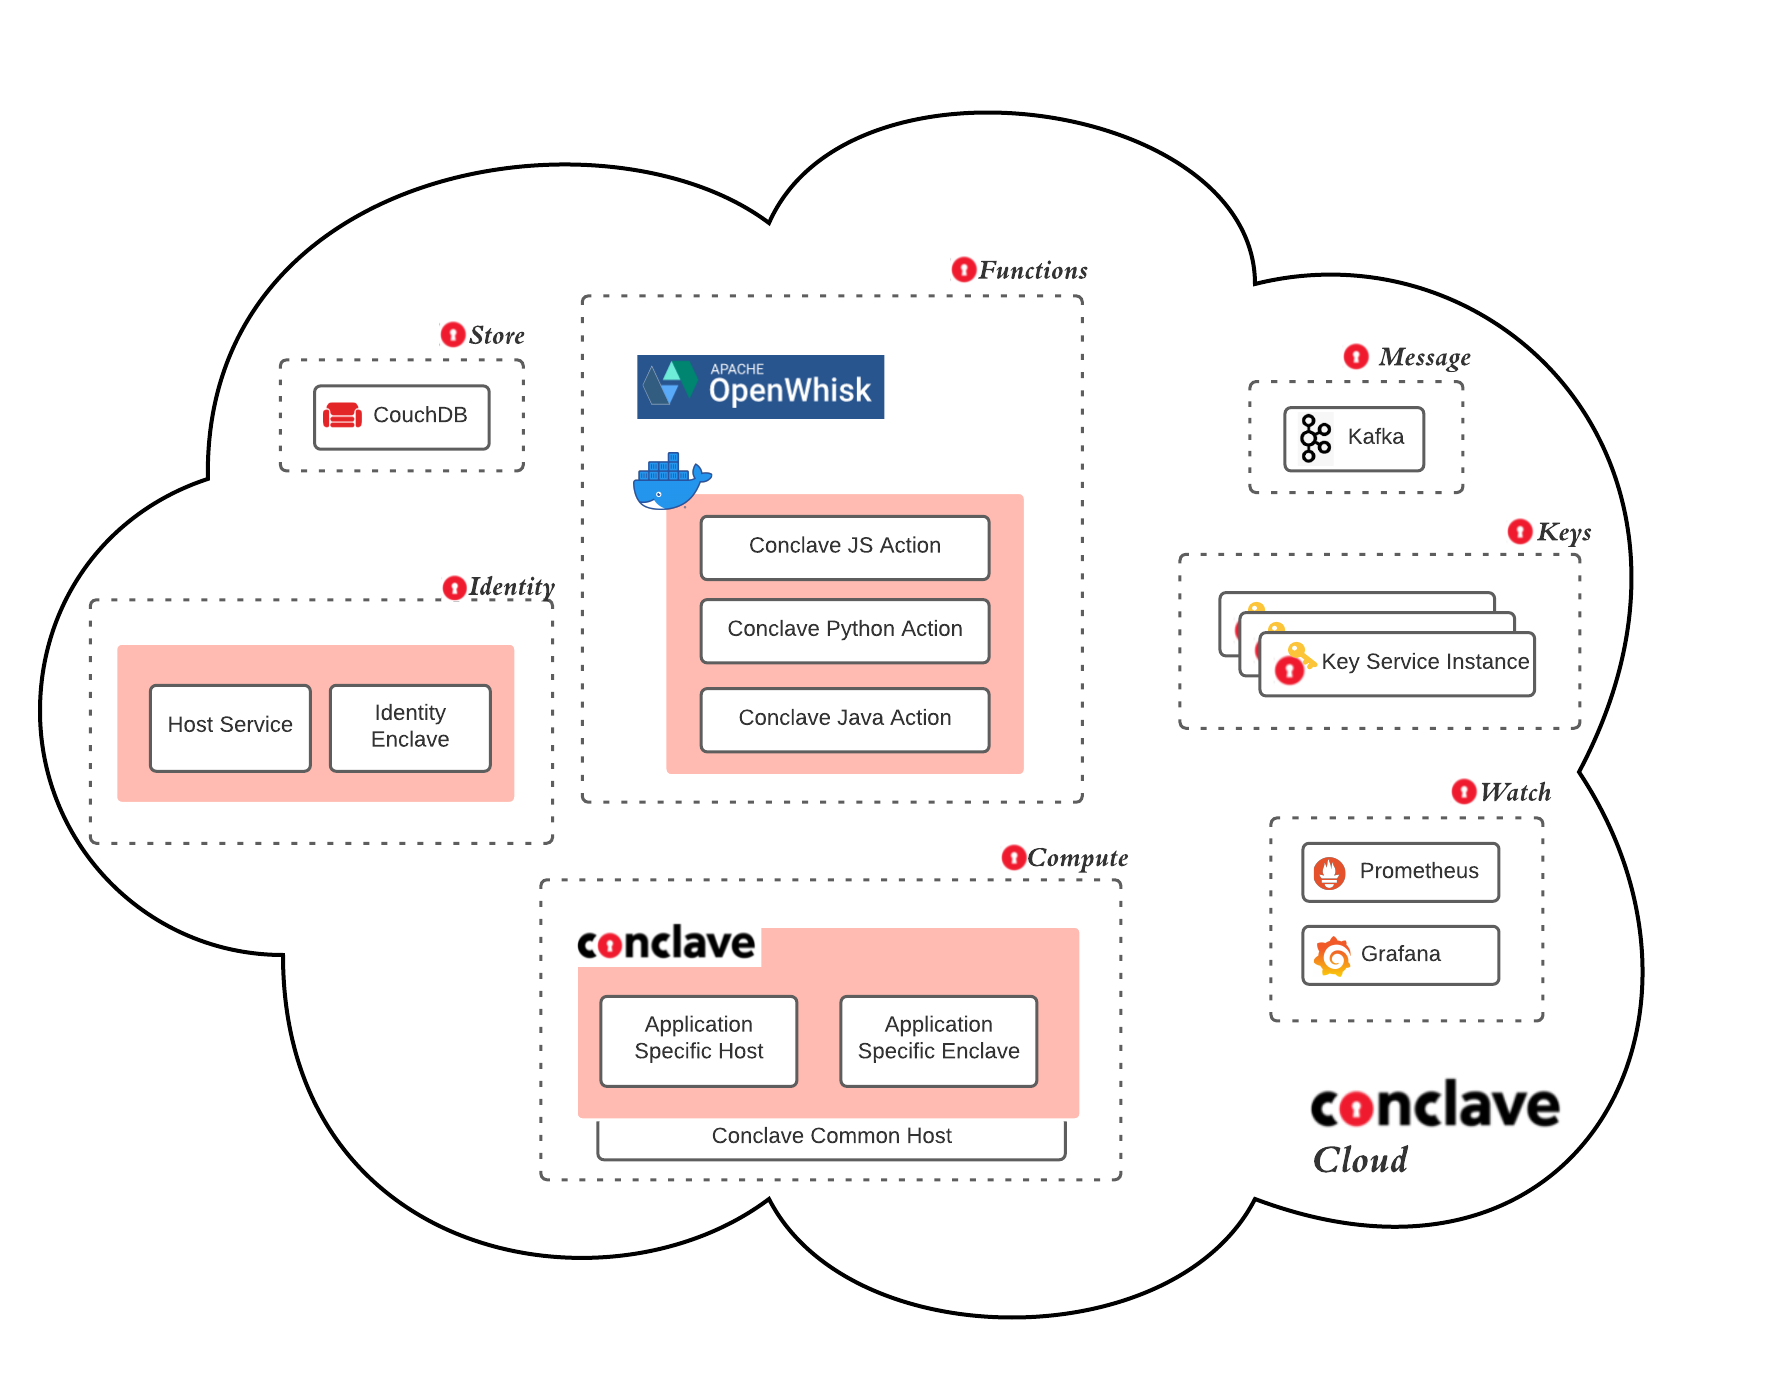
\includegraphics[width=4.64286in,height=3.64047in]{src/media/image7.png}
  \caption{Conclave Cloud is a set of integrated and complementary cloud
  services for the development and execution of privacy-first
  applications, based on Conclave Core}
  \label{image8}
\end{figure}

\hypertarget{key-derivation-and-distribution}{%
\subsubsection{Key Derivation and
Distribution}\label{key-derivation-and-distribution}}

TEEs such as Intel SGX provide support for the secure persistence of
data created by enclaves. But this data can typically only subsequently
be decrypted by the same CPU that encrypted it. This maximises security
but creates a point of failure and is incompatible with deployment in
cloud environments, which typically provide no guarantee that a
particular application will be scheduled to the same CPU from one
invocation to the next.

To solve this problem, Conclave Cloud provides a Key Derivation Service
(KDS). The KDS gives enclave authors complete control over how the data
their enclaves persist is encrypted. This includes the ability to create
encrypted data that can be accessed by other enclaves that are part of
the same enclave `family', facilitating sophisticated architectural
options. In addition, the KDS is fully integrated with Conclave's
support for upgrades to enclaves and the underlying confidential
computing platform. The KDS is agnostic as to the source of the
underlying `master' key used by any given instance of the KDS.
Mainstream deployments of the KDS will likely use keys obtained from a
physical HSM, cloud HSM or a TEE-aware cloud `sealing service' where
available. However, the KDS could also be deployed in a decentralised
mode, where the master key is constructed inside the KDS enclave from a
collection of fragments provided by different parties.

\hypertarget{compute}{%
\subsubsection{Compute}\label{compute}}

Conclave Compute is a managed service for the hosting of enclaves
developed using the Conclave Core Software Development Kit. The Conclave
Core SDK is designed so that all a developer needs to do is write their
enclave business logic, and Conclave Core takes care of instantiating
the enclave and connecting it to clients, with a component known as the
`Common Host'. Conclave Cloud Compute builds on this architecture by
providing a cloud-based Common Host, with additional monitoring and
management logic, providing a seamless path from local test/development
to production-scale operation.

\hypertarget{functions}{%
\subsubsection{Functions}\label{functions}}

The traditional development model for enclave-enabled applications is to
develop an enclave, compile it, and deploy it to a suitable server, at
which point clients can connect, verify its attestation, and begin to
use it. This works well for many classes of application, especially
those where the bulk of the application's logic is custom and/or needs
to run inside a single enclave.

However, there are also many classes of application where the
privacy-first computation is a relatively small (or simple) part of the
overall application, or where the application's design pattern could be
implemented by combining reusable architectural components. We see this
phenomenon in non-private clouds, with the emergence of `micro-service',
`serverless' and `lambda' patterns. What characterises such platforms is
that developers can rapidly compose an application from a palette of
high quality underlying services, such as managed databases, stateless
functions that scale on demand, and so forth.

To meet this demand, Conclave Cloud offers \emph{Functions}, which can
be thought of as a privacy-first analogue of AWS Lambda {[}10{]}.
Specifically: developers can upload one or more functions, written in a
range of languages including Java, JavaScript, Python and more, and
Conclave Cloud will take care of ensuring that the associated functions
can be invoked on demand, automatically scaling the service up and down
as needed. Significantly, Conclave Cloud provides full attestation
capabilities, enabling clients of Conclave Functions to verify that the
function they are invoking exactly matches the function whose source
they have inspected.

\hypertarget{store}{%
\subsubsection{Store and Watch}\label{store}}

Most non-trivial enclaves require persistence. Conclave Cloud provides
both a persistence layer to underpin Conclave Compute, as well as a
fully managed confidential database.

Furthermore, like all managed services, Conclave Cloud is underpinned by a monitoring
and management layer. However, Confidential services present a unique
challenge: the data being processed must remain private, and a common
cause of privacy breaches is the information -- or usage patterns --
that can be revealed from logs. As a result, Conclave Cloud's monitoring
infrastructure -- \emph{Watch} -- has been carefully designed to ensure
that the system can be satisfactorily managed within these constraints.

\hypertarget{comparison-to-software-based-privacy-enhancing-technologies}{%
\section{Comparison to Software-Based `privacy-enhancing'
technologies}\label{comparison-to-software-based-privacy-enhancing-technologies}}

Conclave aspires to be the simplest and most productive platform for
developing privacy-first applications. To achieve this, Conclave builds
on a foundation of industry-standard hardware Trusted Execution
Environments. However, purely software-based techniques also exist. In
this section, we briefly survey the software techniques before outlining
why we believe the Conclave approach is superior.

Conclave's primary differentiators with respect to those techniques are
as follows:

\begin{itemize}
\item
  Unlike the software-based techniques, Conclave applications can be
  created by developers with `off-the shelf' skills. No advanced
  training in cryptography or mathematics is required.
\item
  In addition, Conclave provides `remote attestation' as an integral and
  out-of-the-box feature, meaning that, unlike Fully Homomorphic
  Encryption solutions, Conclave can provide assurances that not only is
  data protected when in the hands of a third party but it is possible
  to verify what algorithm they actually ran on it
\item
  And Conclave's high-level APIs, which are tightly integrated with each
  other and seamlessly available across Conclave Cloud's services, fully
  abstract the details of the underlying hardware Trusted Execution
  Environments. This means that Conclave developers do not need to
  invest resources in understanding -- and keeping pace with -- advances
  in the underlying technology. This contrasts strongly with users of
  software-based cryptographic techniques, who must keep up with
  extremely rapid advances.
\end{itemize}

In what follows, we introduce the main software-based techniques and
develop the argument for why we believe Conclave's approach is superior.

\hypertarget{background-1}{%
\subsubsection{Background}\label{background-1}}

As discussed above, hardware-based techniques, such as Conclave, attack
the `trust' problem at source: they make it possible to build trust in
what will happen to your information when processed on a third party's
computer.

The software-based mathematical techniques outlined in this section take
a different approach. Their starting point is that if you can't trust
somebody else's computer yet nevertheless need to cooperate with them
for some purpose, then we need to radically limit what information is
shared. And the techniques we will discuss are the result of exploring
this thought process, focusing here on solutions that are enabled
through advanced cryptography\footnote{Software techniques that do not
  depend on cryptography also exist and are widely deployed. They employ
  techniques such as obfuscating records, injecting `decoy' data or
  simply eliminating entire columns of data. However, this means they
  are inherently 'lossy', and so we do not discuss them further/}.

However, and as we will also go on to demonstrate, it turns out that the
specialised problems that pure software-based techniques can solve can
\emph{also} be solved by Conclave This underpins our claim that any firm
for whom a software-based privacy-enhancing technique meets their needs
could immediately switch to Conclave to achieve the same security
benefit but with radically quicker deployment times and radically lower
implementation costs.

It should also be noted that all of these techniques significantly
reduce the amount of trust one party need have on any other party, but
none can totally eliminate the need for some elements of trust. For
example, and as we will outline below, users of Trusted Execution
Environments must trust that the vendor of the CPU has implemented it
correctly and honestly. Similarly, non-specialist users of cryptographic
techniques need to trust both that the underlying algorithms are indeed
secure and that they have been implemented correctly.

The software-based techniques turn out to be more specialised and
narrowly applicable than the more general-purpose hardware approach.
However, it turns out that the different approaches map well to the
use-cases outlined earlier and so we structure what follows in a similar
manner.

\hypertarget{outsourced-computation-1}{%
\subsubsection{Outsourced Computation}\label{outsourced-computation-1}}

Imagine you have a list of numbers and you wanted to know the sum, for
example, and wanted somebody else to calculate it for you. But you
didn't want them to be able to see the numbers themselves. A technique
known as \emph{\textbf{Fully Homomorphic Encryption}, or FHE} {[}6{]}
allows you to encrypt the list, send it to a third party, and for the
third party to perform the calculations you asked for on the encrypted
data, yielding some encrypted result which, when you decrypt it, is the
answer to your question.

However, there is no way to know that the result you get back really
\emph{was} the result of the computation you requested. Perhaps the
service provider only summed every \emph{other} integer. You have no way
of knowing, aside from re-running the computation yourself, so it turns
out that the applicability of FHE may be fairly limited, even when it is
applicable, which is only in specific circumstances and when the
performance overhead is not an issue.

\hypertarget{independent-verification}{%
\subsubsection{Independent
Verification}\label{independent-verification}}

The second major software-based technique concerns itself with answering
the question: ``if I possess something that you would believe if you
could see it, can I convince you of something \emph{derived} from it
without you learning anything else at all''?

\emph{\textbf{Zero Knowledge Proofs}, or ZKPs} {[}7{]}\emph{,} make it
possible to mathematically prove a fact about a secret piece of
information without revealing anything aside from that fact. And it is
perhaps no surprise that zero knowledge proofs have become such an
active research field at the same time as the rise of blockchains: if I
can prove to you that I own a coin without having to reveal to you how I
came to own it, you might be willing to accept it as payment without
needing to know anything about my transaction history or how I came to
own it. It would turn the very traceable world of public
cryptocurrencies into something far more `cash-like'.

However, ZKPs do not, at present, appear to be ready for mainstream
adoption in business. There is no general-purpose, easy to use,
technique for generating zero knowledge proofs about arbitrary facts,
the technology changes rapidly, and `generation' of proofs can be
extremely slow.

\hypertarget{multi-party-collaboration-1}{%
\subsubsection{Multi-Party
Collaboration}\label{multi-party-collaboration-1}}

The field of ``\textbf{Secure Multi-Party Computation}'', or sMPC
{[}8{]}, is based on the idea that sometimes there are ways to
\emph{distribute} the processing that needs to be done on behalf of a
group of parties so that each party runs their own part of the
computation and then the results, which don't contain the input data in
an easy to recover form, can then be combined to yield the result.
However, like ZKPs, the technology is not yet generally applicable or
easily usable by ordinary developers and, like FHE, there's no way to
know whether your counterparts played fair: did they \emph{really}
follow their parts of the process correctly?

\hypertarget{discussion}{%
\subsubsection{Discussion}\label{discussion}}

One advantage of the software-based techniques is that by being rooted
in deep mathematical theory and by working on existing hardware, they do
not require the introduction of a new trusted party into the equation,
at least not obviously. Further weighing to their advantage is that
these techniques are rapidly advancing.

However, their downside is their complexity, lack of general
applicability, performance, and the problem that each of them only
solves one part of the puzzle when, quite often, what you need is a
simple solution that can be deployed rapidly and which addresses two or
even three of the requirements above at the same time. For example, if I
outsource computation to the cloud, I want to know \emph{both} that my
data is secure \emph{and} that the results I receive really \emph{were}
the output of the query I ran. To achieve that with a software technique
would require me, somehow, to combine a general---purpose fully
homomorphic encryption solution with a zero knowledge proof. Mathematics
will get there, but it's not there yet.

In Figure 4, we summarise the high-level breakdown outlined above,
distinguishing between hardware- and software-based techniques and,
within the software techniques, further breaking out the three most
prevalent cryptographic approaches.

\begin{figure}
  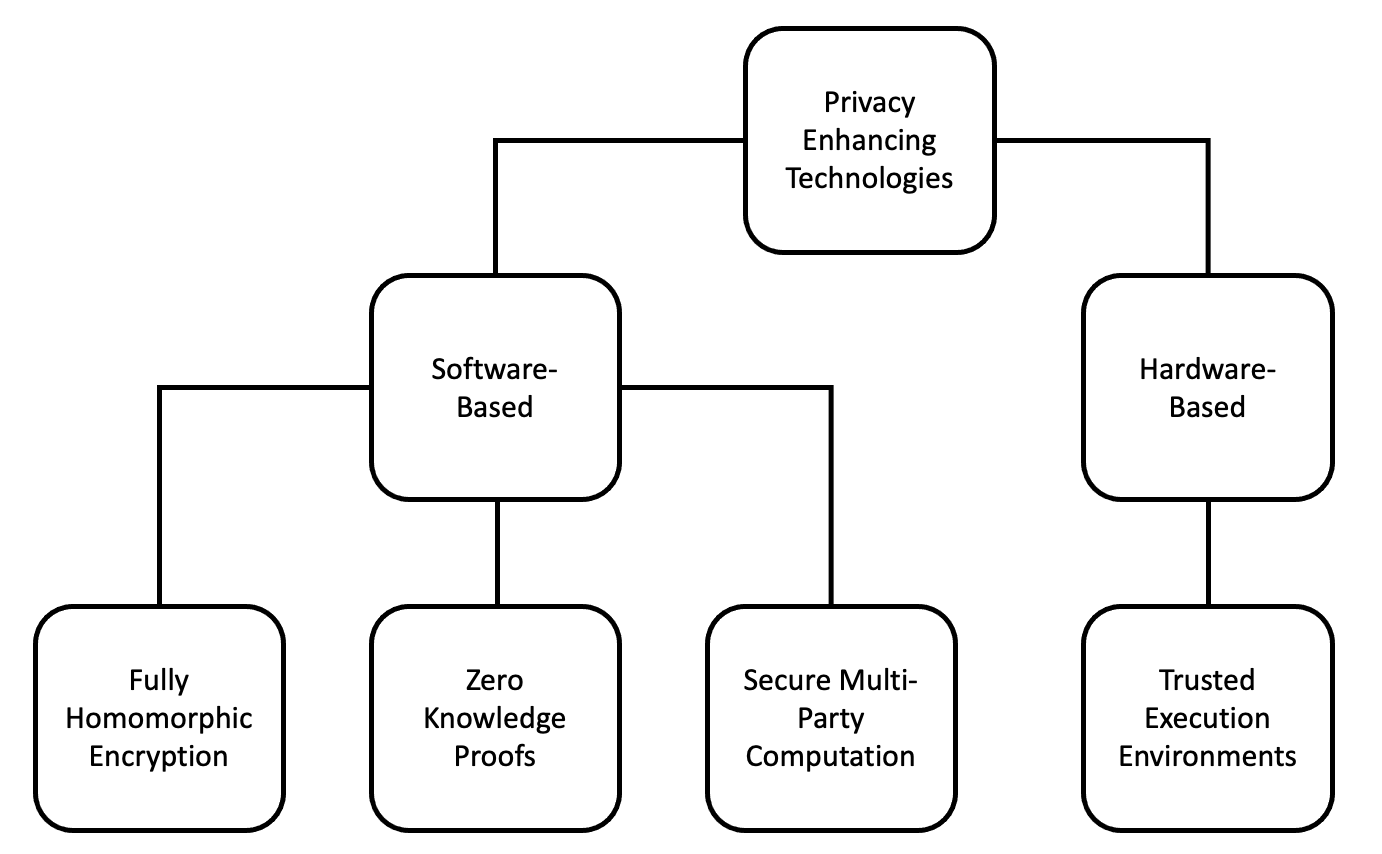
\includegraphics[width=4.5625in,height=2.81944in]{src/media/image8.png}
  \caption{It can be convenient to distinguish between software-based and
  hardware-based technologies for enhancing the privacy of IT solutions}
  \label{image6}
\end{figure}

At first glance, hardware based techniques may appear to be superior in
every way to the software techniques: a unified approach rather than
three distinct research fields; minimal performance overheads; far fewer
limitations and special cases.

And on a practical day-to-day basis, this is true. However, in the
interest of balance, it is worth highlighting two significant objections
to the use of TEEs. First, without a solution such as Conclave they can
be surprisingly tricky to program, especially to program securely. This
is because they turn programmers' assumptions about the role of
different system components on their heads. For example, and as
discussed above, TEE programmers cannot assume an operating system
kernel is trusted. Conclave is intended to address this cognitive and
productivity problem, and this is what we believe tilts the balance
decisively against the software-based techniques.

And it can also be argued that TEEs introduce a new actor into the
threat model: the vendor of the underlying hardware technology. For
example, if you use the Intel SGX TEE then you are directly dependent on
the integrity of Intel's development processes and its ability to
withstand pressure from one or more state actors to incorporate `back
doors' into its chips. However, it is also worth observing that the
software techniques also run on hardware and so if a malicious CPU
manufacturer is in your threat model then you need to carefully consider
which attacks you may be exposed to even when using software techniques,
even if the risk may be lower.

\hypertarget{threat-model}{%
\section{Threat Model}\label{threat-model}}

Conclave adopts the Confidential Computing Consortium's threat model
{[}12{]}. We start by assuming one or more clients, each trusted by
their users, are seeking to communicate with a program whose source they
have verified or whose author they trust, which we call an enclave.
However, we assume that the computer on which this enclave is running
may be operated by an adversary who seeks to subvert the operation of
the program and/or observe the plaintext on which it operates.

This malicious operator is assumed to have control of all hardware
outside the CPU package, all software outside the enclave, and of any
devices to which the computer is connected, including any storage or
network devices. This means the adversary has the ability to block,
reorder or replay messages; to observe any data which enters or leaves
the enclave; to delete or replace any data sent to/from storage; to
observe the behaviour of the system as it performs its work, including
its CPU utilisation and temperature; and to restart or otherwise
interrupt the execution of the enclave, including by disrupting or
altering its power or otherwise injecting faults.

However, whilst we assume the adversary has physical access to the
computer, we do not assume that the adversary has the ability to observe
the CPU at the atomic or sub-atomic level. As such, we assume that any
secret keys `burned' into CPUs at the time of manufacture upon which
they depend for their secure operation cannot be recovered.

Furthermore, we do not include the host's trivial ability to deny
service by failing to schedule an enclave for execution in our threat
model.

It should be noted, however, that any given Conclave application may not
face a threat model as stringent as this and, as such, may not require
all the protections that Conclave provides, or contemplates providing in
the future. To that end, Conclave provides some features that developers
can elect to use that do not mitigate all these threats, but whose
utility is high enough to make the tradeoff acceptable. A notable
example is Conclave's encrypted file-system which, by itself, is not
secure against `rewind attacks', but which can be made so by using it in
combination with the `persistent map.'

\hypertarget{conclusion}{%
\section{\texorpdfstring{Conclusion }{Conclusion }}\label{conclusion}}

We have presented Conclave, a platform for the rapid development and
execution of `privacy-first' services and a set of privacy-first cloud
services that are themselves built using the Conclave platform.

Conclave puts the power of Trusted Execution Environments into the hands
of developers, enabling them to write privacy-first applications with
ease, using the productive high-level languages they're already using to
develop their existing solutions.

Conclave's productivity and ease of use stands in contrast to the
learning curve associated with competing software-based cryptographic
approaches. And Conclave distinguishes itself from competing
hardware-focused platforms through the speed with which developers
familiar with languages such as Java, JavaScript, Kotlin and Python can
develop compelling, privacy-first applications.

Conclave enables users to build, deploy and integrate privacy-first
services at scale and, in so doing, heralds the mainstream era of
`privacy-first' computation.

\newpage
\hypertarget{bibliography}{%
\section{Bibliography}\label{bibliography}}
% If this section ever grows to more than one page, it will need to be fixed (you'll see why...)
% Also - should really be turned into a proper bibtex
\begin{longtable}[]{@{}
  >{\raggedright\arraybackslash}p{(\columnwidth - 2\tabcolsep) * \real{0.0517}}
  >{\raggedright\arraybackslash}p{(\columnwidth - 2\tabcolsep) * \real{0.9483}}@{}}
\toprule
\begin{minipage}[b]{\linewidth}\raggedright
{[}1{]}
\end{minipage} & \begin{minipage}[b]{\linewidth}\raggedright
Intel, ``Intel Software Guard Extensions,'' 2021. {[}Online{]}.
Available:
https://www.intel.com/content/www/us/en/developer/tools/software-guard-extensions/overview.html.
\end{minipage} \\
%\midrule
\endhead
{[}2{]} & BBC, 2020. {[}Online{]}. Available:
https://www.bbc.co.uk/news/technology-54722362. \\
{[}3{]} & Apple, 2021. {[}Online{]}. Available:
https://www.apple.com/privacy/docs/A\_Day\_in\_the\_Life\_of\_Your\_Data.pdf. \\
{[}4{]} & ICO, 2021. {[}Online{]}. Available:
https://ico.org.uk/for-organisations/guide-to-data-protection/guide-to-the-general-data-protection-regulation-gdpr/lawful-basis-for-processing/consent/. \\
{[}5{]} & Bloomberg, 2021. {[}Online{]}. Available:
https://www.bloomberg.com/news/articles/2021-11-08/robinhood-data-breach-exposes-data-on-millions-of-customers. \\
{[}6{]} & Red Hat, 2019. {[}Online{]}. Available:
https://next.redhat.com/2019/12/02/current-trusted-execution-environment-landscape/. \\
{[}7{]} & Oracle, 2021. {[}Online{]}. Available:
https://www.graalvm.org/. \\
{[}8{]} & Amazon, 2021. {[}Online{]}. Available:
https://aws.amazon.com/lambda/. \\
{[}9{]} & IBM, 2021. {[}Online{]}. Available:
https://research.ibm.com/labs/uk/fhe.html. \\
{[}10{]} & K. Chalkias, 2017. {[}Online{]}. Available:
https://www.linkedin.com/pulse/demonstrate-how-zero-knowledge-proofs-work-without-using-chalkias/. \\
{[}11{]} & Inpher, 2021. {[}Online{]}. Available:
https://inpher.io/technology/what-is-secure-multiparty-computation/. \\
{[}12{]} & CCC, 2020. {[}Online{]}. Available:
https://confidentialcomputing.io/wp-content/uploads/sites/85/2020/10/Confidential-Computing-Deep-Dive-white-paper.pdf. \\
\bottomrule
\end{longtable}

\hypertarget{acknowledgements}{%
\section{Acknowledgements}\label{acknowledgements}}

The author is grateful to Ivar Wiersma, Rusheb Shah, Rui Almeida, Roy
Hopkins, Sneha Damle and Shams Asari for valuable feedback on earlier
drafts of this paper. The design of Conclave was a team effort, led by
Mike Hearn, Shams Asari and Roy Hopkins.

\end{document}
